\documentclass[a0, portrait]{a0poster}
%%%Load packages
\usepackage{multicol} 			%3-column layout
\usepackage[left=1.5cm,right=1.5cm,bottom=0cm,top=0cm]{geometry}			%Reset margins
%\usepackage{fontspec} % For loading fonts
%\setmainfont[SmallCapsFont = Fontin SmallCaps, Ligatures=TeX]{Fontin} % Main document font
\usepackage[scaled=1]{helvet}
\usepackage[x11names]{xcolor}				%Needed for colour boxes & coloured text
\usepackage{graphicx}%%%Define colours and lengths
\usepackage[export]{adjustbox}
\usepackage{authblk}
\usepackage{amsmath} % Equations
\usepackage{amssymb} % Equations
\usepackage{bbm} %mathbbm
\usepackage{anyfontsize}
\usepackage{array, booktabs}
\usepackage[utf8]{inputenc}
\usepackage{tcolorbox}
\usepackage{mathtools}
\usepackage[hidelinks, linktoc=all, russian]{hyperref}
\usepackage{cleveref}
\usepackage{capt-of}
\usepackage[font=small,labelfont=bf]{caption}
\usepackage{subcaption}
\captionsetup[subfigure]{labelformat=parens}

\definecolor{headingcol}{rgb}{0.4, 0.57, 0.83}			%Colour of main title
\definecolor{titlecol2}{HTML}{CC181E}			%Colour of main title

\definecolor{titlecol}{rgb}{0.3, 0.47, 0.73}			%Colour of main title
\definecolor{boxcol}{rgb}{0.7,0.2,0.2}		%Edge-colour of box and top banner
\fboxsep=1cm							%Padding between box and text
\setlength{\columnsep}{2cm}				%Set spacing between columns
\renewcommand{\familydefault}{\sfdefault}	%Set main text to sans-serif


\newenvironment{frshaded}{%
	\def\FrameCommand{\fboxrule=\FrameRule\fboxsep=\FrameSep \fcolorbox{framecolor}{shadecolor}}%
	\MakeFramed {\FrameRestore}}%
{\endMakeFramed}

\renewcommand{\figureautorefname}{Fig.}%
\renewcommand{\figurename}{Fig.}

\graphicspath{{Pictures/}}

\newcommand{\diff}{\,\mathrm{d}} 	
\renewcommand{\figureautorefname}{Fig.}%
\renewcommand*\thesection{\arabic{section}}
\DeclarePairedDelimiter\bra{\langle}{\rvert}
\DeclarePairedDelimiter\ket{\lvert}{\rangle}
\DeclarePairedDelimiterX\braket[2]{\langle}{\rangle}{#1 \delimsize\vert #2}
\newcommand{\rbrkt}[1]{\left( #1 \right)}
\newcommand{\sbrkt}[1]{\left[ #1 \right]}

\begin{document}

\begin{center}
\vspace*{-2cm}
\hspace*{-2cm}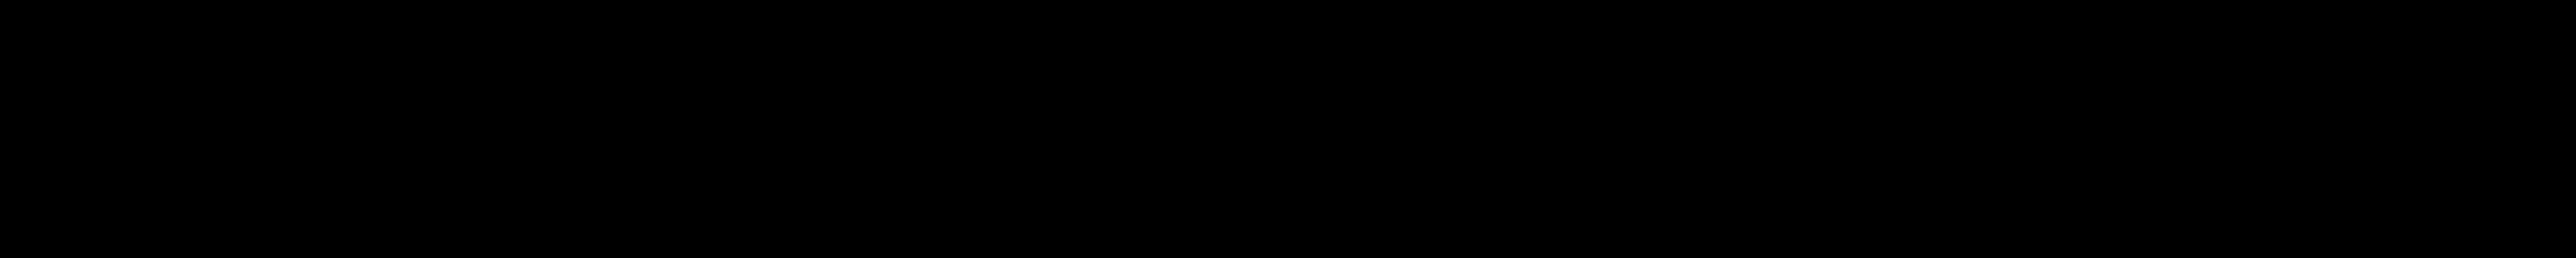
\includegraphics[width=1.2\textwidth]{Black_Landscape}
\end{center}


%%% Title
\begin{minipage}{0.65\textwidth}					
\vspace{-11cm}
\begin{tabular}[t]{l}
{\color{headingcol}\fontsize{68}{70}\selectfont Analog Ising chain simulation with transmons}\\
\\
{\hspace{0.2cm} \color{white}\large  E. Egorova\textsuperscript{1,2}, G. Fedorov\textsuperscript{1,2,4}, A. Dobronosova\textsuperscript{3}, N. Orlikovskiy\textsuperscript{3} and A. V. Ustinov\textsuperscript{1,4,5}} \\
\\
{\hspace{0.2cm}\color{white}\large \hspace{0.5cm} \textsuperscript{1}\textit{Russian Quantum Center} \hspace{0.5cm} \textsuperscript{2}\textit{Moscow Institute of Physics and Technology} \hspace{0.5cm} 
\textsuperscript{3}\textit{Bauman MSTU} \hspace{0.5cm}}\\ 
{\color{white}\large \hspace{0.5cm}\textsuperscript{4}\textit{National University for Science and Technology MISiS} \hspace{0.5cm} 
\textsuperscript{5}\textit{Karlsruhe Institute of Technology}}
\end{tabular}
\end{minipage}
%%% Logos
\hspace{19cm}
\begin{minipage}{0.2\textwidth}
\vspace{-11cm}
\begin{tabular}{c c}

\includegraphics[height=0.05\textheight]{log}
\end{tabular}
\end{minipage}


\vspace{-1.5cm}
\begin{multicols}{2}	

%%%Column1

%%%%%%%%%%%%%%%%%% Introduction

\tcbset{colframe=titlecol, colback=white}
\begin{tcolorbox}[left=1cm, right=1cm, top=0.5cm, bottom=0.5cm, 
                  title={\Large Introduction}, bottomtitle=.5cm,toptitle=.5cm]
\begingroup
\setlength{\columnsep}{1cm}
Currently, the applications of medium-scale systems composed of superconducting qubits are mostly limited to testing basic principles of quantum computation, demonstrating those as proof-of-concept designs and developing scalable software and hardware interfaces to them. Although this is useful in terms of encouraging future developments in the domain, an alternative approach exists to exploit the built-in quantum properties of such devices to experiment with fundamental physical models. There already were\cite{li2018perfect}\cite{macha2014implementation}\cite{roushan2017spectroscopic} some successful attempts to use small arrays of superconducting qubits to observe inherently quantum analog behaviour of these systems, and this work is aimed to continue those studies. We are developing a chip to experimentally simulate crystal structure, many-body localization and heat transport properties with a chain of XX-coupled transmons.
\endgroup
\end{tcolorbox}

%%%%%%%%%%%%%%%%%% Idea

\tcbset{colframe=titlecol}
\begin{tcolorbox}[left=1cm, right=1cm, top=0.5cm, bottom=0.5cm, 
                  title={\Large Study concept}, bottomtitle=.3cm,toptitle=.5cm
                  ]
		The Hamiltonian of five transmons interacting only with the nearest neighbors can be written as the sum of the Hamiltonian of the transmons without and with the interaction:               
		
		$$\hat{H}_{full} = \sum_{i=1}^5 \hat{1}_1 \otimes \hat{1}_2 \otimes...\otimes \hat{H}_{i_0} \otimes...\otimes \hat{1}_5 +  \sum_{i=1}^{4} \frac{e^2 M^{-1}_{i,j=i+1}}{2} \hat{1}_1 \otimes \hat{1}_2 \otimes...\otimes \hat{n}_{i} \otimes \hat{n}_{j} \otimes...\otimes \hat{1}_5,
		$$ 
		Here $\hat{H}_{i_0}$ - single transmon Hamiltonian, and $M^{-1}_{i,j=i+1}$ - inverse capacity matrix element.
		Ising Hamiltonian can be written as $$
		H = -\frac{1}{2}\sum_{i}h_i\sigma_{z,i}+\hbar\sum_{i}J_{x,i}\sigma_{x,i}\sigma_{x,i+1},
		$$ where $
		J_{y,i},J_{z,i}=0
		$. Since two above-described Hamiltonians have a similar structure, it becomes possible to carry out analog modeling of the spin chain.
		\\At the same time we can write Hamiltonian of five-resonator chain using classical mechanics: $$
		\hat{H}_{cl} = \sum_{i=0}^{4} \bigg(\frac{\varphi_i^2}{2L_i} + \frac{q_i^2 M^{-1}_{i,i}}{2} \bigg) + \sum_{i=0}^{3} M^{-1}_{i,i+1}q_i q_{i+1}.
		$$
		 
\end{tcolorbox}


%%%%%%%%%%%%%%%%%% Sample design
\tcbset{colframe=titlecol}
\begin{tcolorbox}[left=1cm, right=1cm, top=0.5cm, bottom=0.5cm, 
                  title={\Large Design}, bottomtitle=.3cm,toptitle=.5cm
                  ]

\vspace{1cm}
\begin{minipage}{\textwidth}
\centering
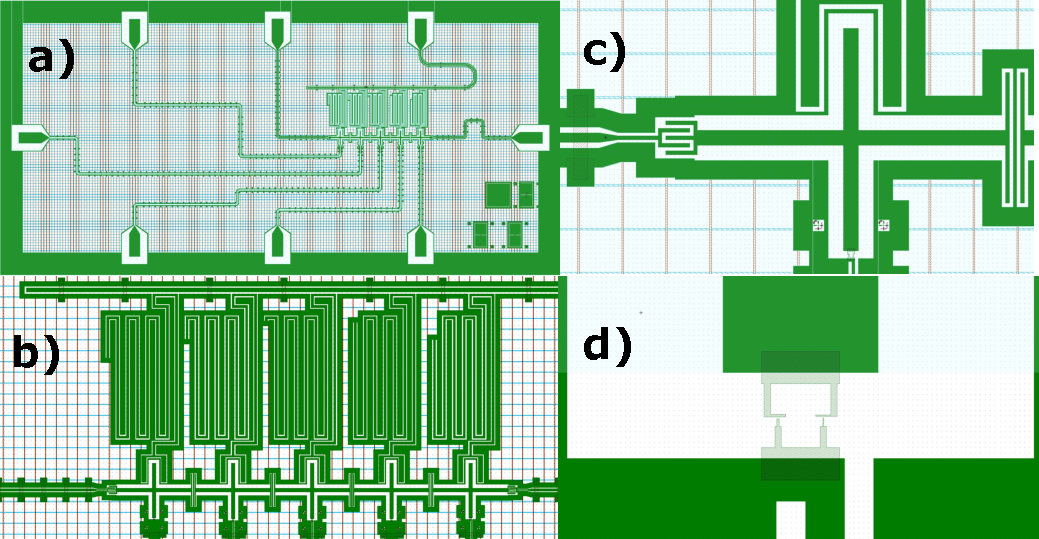
\includegraphics[width=\textwidth]{design}
\begingroup
\captionsetup[figure]{width=\textwidth}

\captionof{figure}{\textbf{(a)} Sample design: 5-transmon chain with XX-coupling; 5 resonators and flux-bies lines; 2 microwave drive lines(for 1st and 5th qubits). \textbf{(b)} \textbf{(c)}\textbf{(d)} Zoomed areas with resonators, microwave antenna and SQUID respectively.}
\endgroup
\end{minipage}

\end{tcolorbox}



%%%%%%%%%%%%%%%%%% Моделирование в Максвелле
\tcbset{colframe=titlecol}
\begin{tcolorbox}[left=1cm, right=1cm, top=0.5cm, bottom=0.5cm, 
	title={\Large ANSYS Maxwell capacitances simulation}, bottomtitle=.3cm,toptitle=.5cm
	]
\begin{minipage}{\textwidth}

	To control the interaction with the nearest neighbors mainly and relaxation in microwave drive antenna, the calculation of the capacitancies of the design was carried out.

\end{minipage}
	
	\vspace{1cm}
	\centering

\begin{minipage}{\textwidth}
	\begin{minipage}{0.4\textwidth}
		\centering
		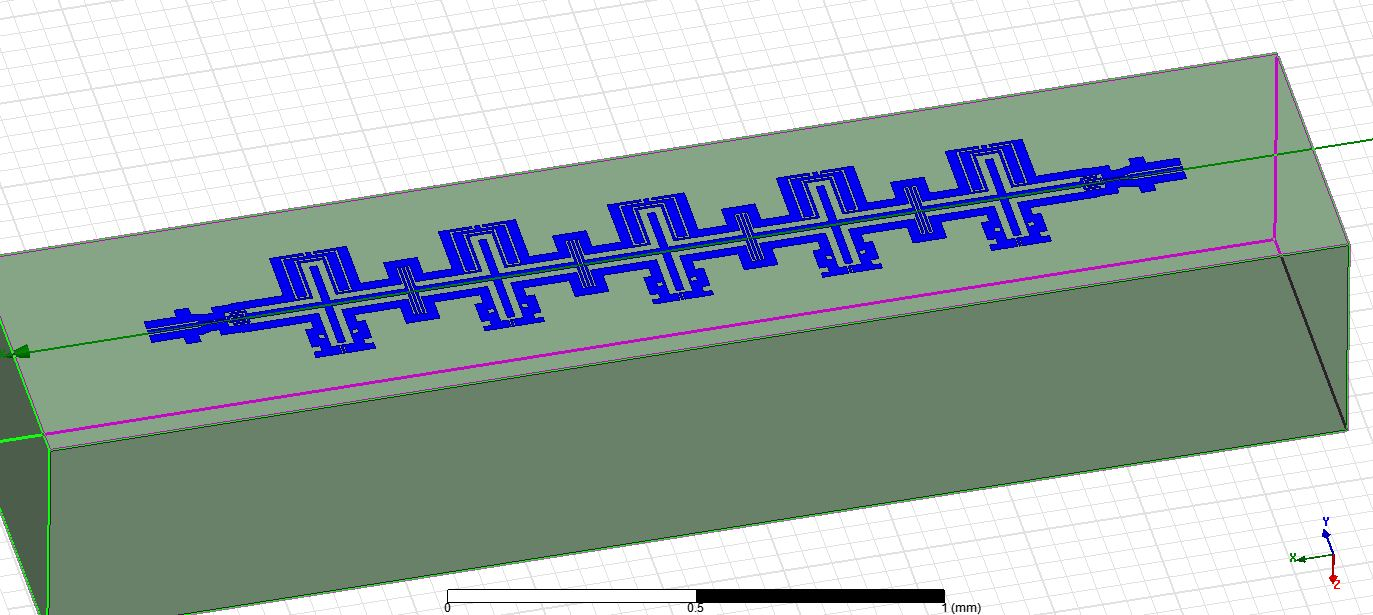
\includegraphics[width=\textwidth]{maxwell_des}
		\begingroup
		\captionsetup[figure]{width=\textwidth}
		
		\captionof{figure}{Calculation of capacitancies by the finite element method.}
		\endgroup
	\end{minipage}
	\begin{minipage}{0.6\textwidth}
		\centering
		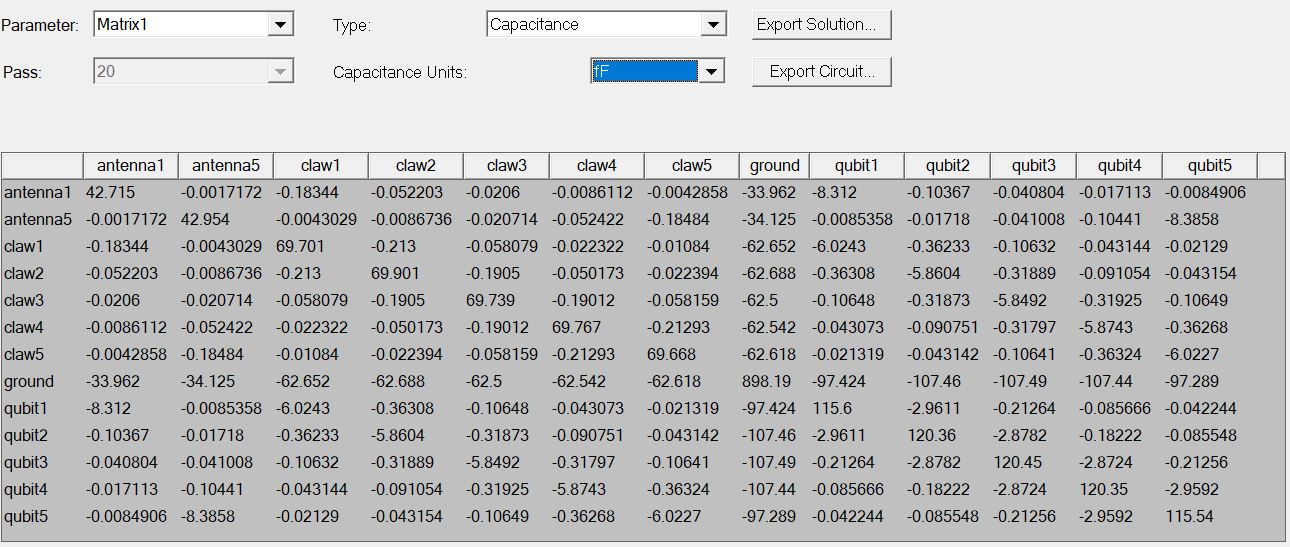
\includegraphics[width=\textwidth]{maxwell_cap}
		\begingroup
		\captionsetup[figure]{width=\textwidth}
		
		\captionof{figure}{The table with obtained capacitancies.}
		\endgroup
	\end{minipage}
\end{minipage}
	
\end{tcolorbox}

\tcbset{colframe=titlecol}
\begin{tcolorbox}[left=1cm, right=1cm, top=0.5cm, bottom=0.5cm, 
	title={\Large Relaxation in antenna}, bottomtitle=.3cm,toptitle=.5cm
	]
	\begin{flushleft}
	To make relaxation rate of chain in transmission line predominant we made sufficient capacitance between them and calculated this rate using formula $Im(\omega)=\frac{1}{2R^*C}$, where $R^* = \frac{1+\omega^2C_k^2Z_0^2}{\omega^2C_k^2Z_0}$ and $C^* = \frac{C_k}{1+\omega^2C_k^2Z_0^2} \simeq C_k$ 
	\end{flushleft}
	\begin{minipage}{0.8\textwidth}
		\centering
		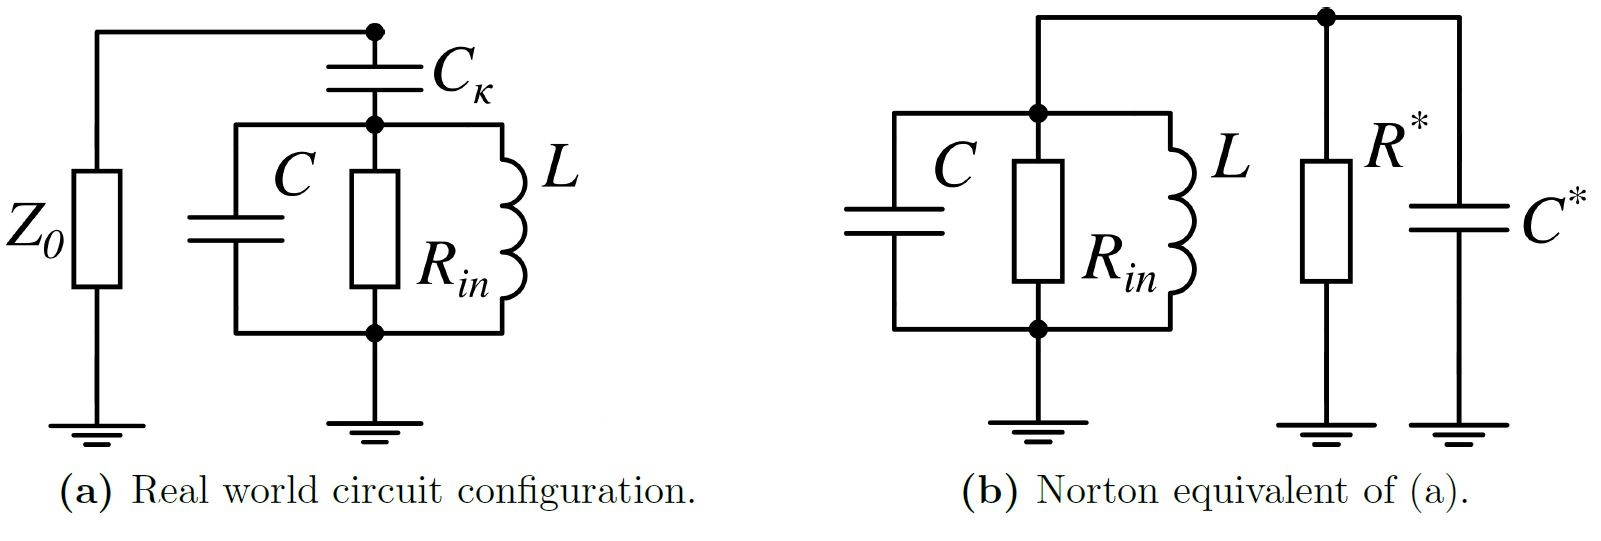
\includegraphics[width=\textwidth]{relaxation}
		\begingroup
		\captionsetup[figure]{width=\textwidth}
		
		\captionof{figure}{Equivalent circuit for a $\lambda/4$ TLR(transmission line resonator), capacitively coupled to the transmission line near resonance.}
		\endgroup
	\end{minipage}
	
\end{tcolorbox}




%%%%%%% Классега
\tcbset{colframe=titlecol}
\begin{tcolorbox}[left=1cm, right=1cm, top=0.5cm, bottom=0.5cm, 
	title={\Large Dynamics simulation. Classical approach}, bottomtitle=.3cm,toptitle=.5cm
	]
	\begin{minipage}{\textwidth}
		
		We made calculation of chain resonant frequencies in LTspice program without and with inductance spread:
		
	\end{minipage}
	
	\begin{minipage}{0.49\textwidth}
		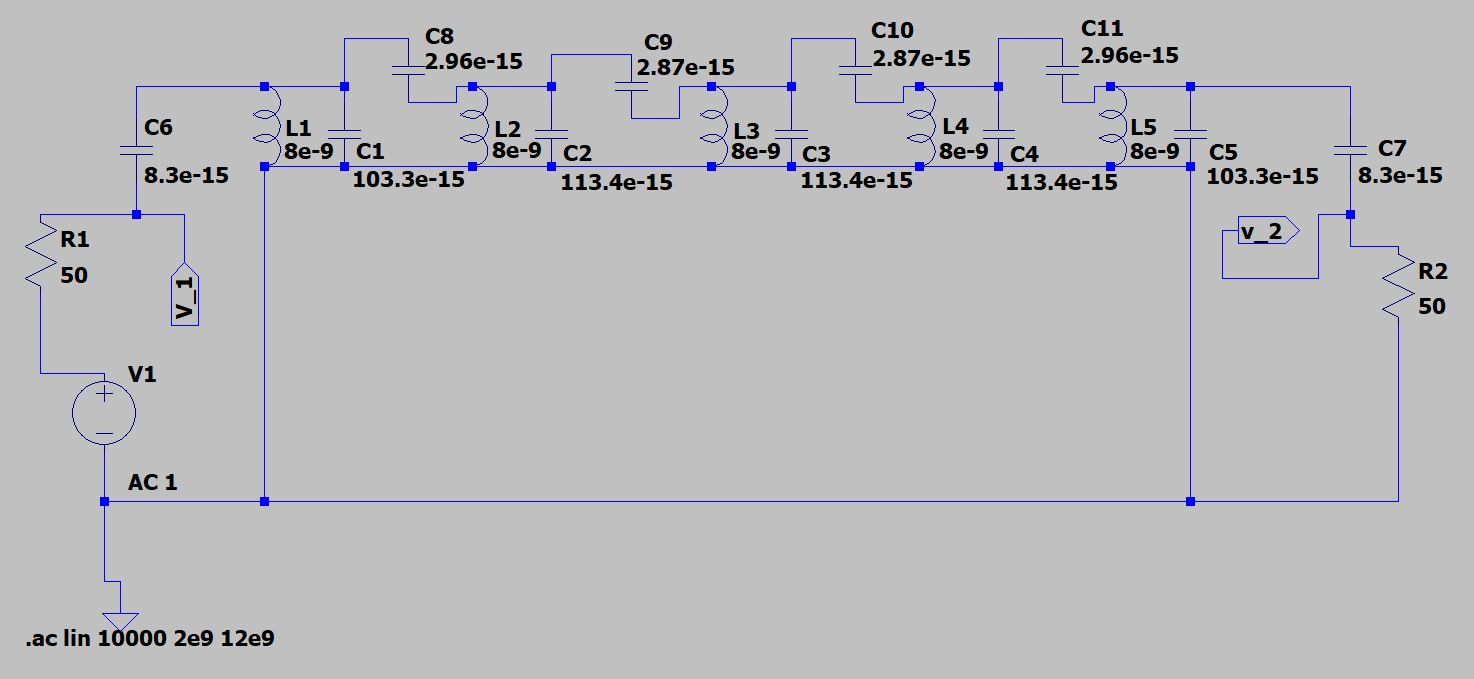
\includegraphics[width=\textwidth]{LTSpice_scheme}
		
		\begingroup
		\captionsetup[subfigure]{width=0.8\textwidth}
		\captionof{subfigure}{Electrical circut scheme in LTspice with equal inductancies}
		\endgroup
	\end{minipage}
	\begin{minipage}{0.49\textwidth}
		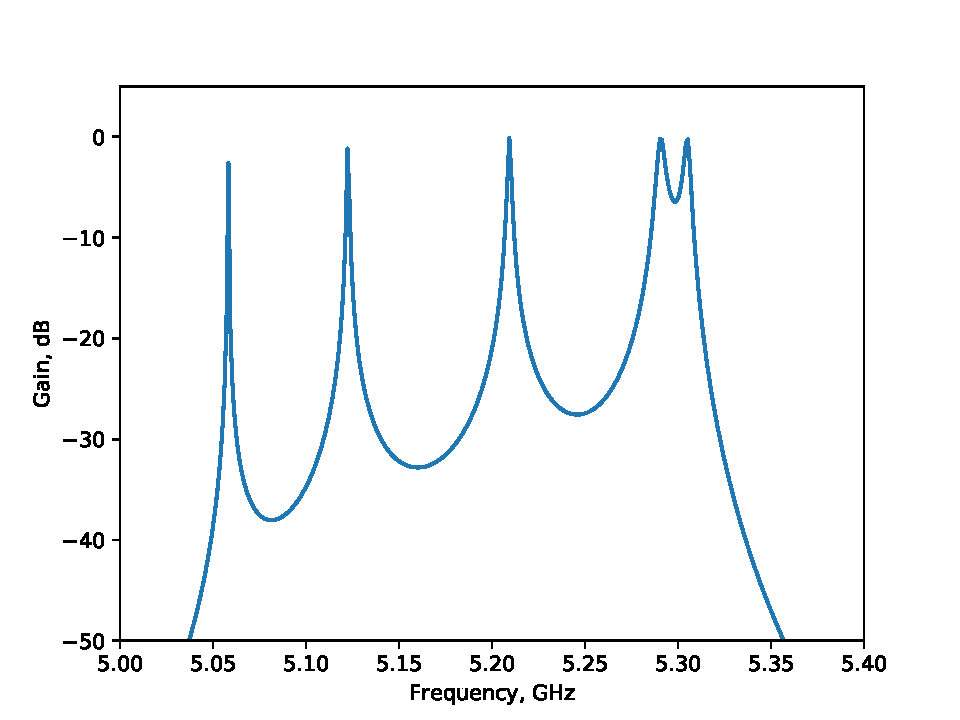
\includegraphics[width=\textwidth]{LTSpice_python_b}
		
		\begingroup
		\captionsetup[subfigure]{width=0.8\textwidth}
		\captionof{subfigure}{Classical mode frequencies in GHz: \{5.059, 5.124, 5.21, 5.291, 5.306\}}
		\endgroup
	\end{minipage}

	\begin{minipage}{0.49\textwidth}
	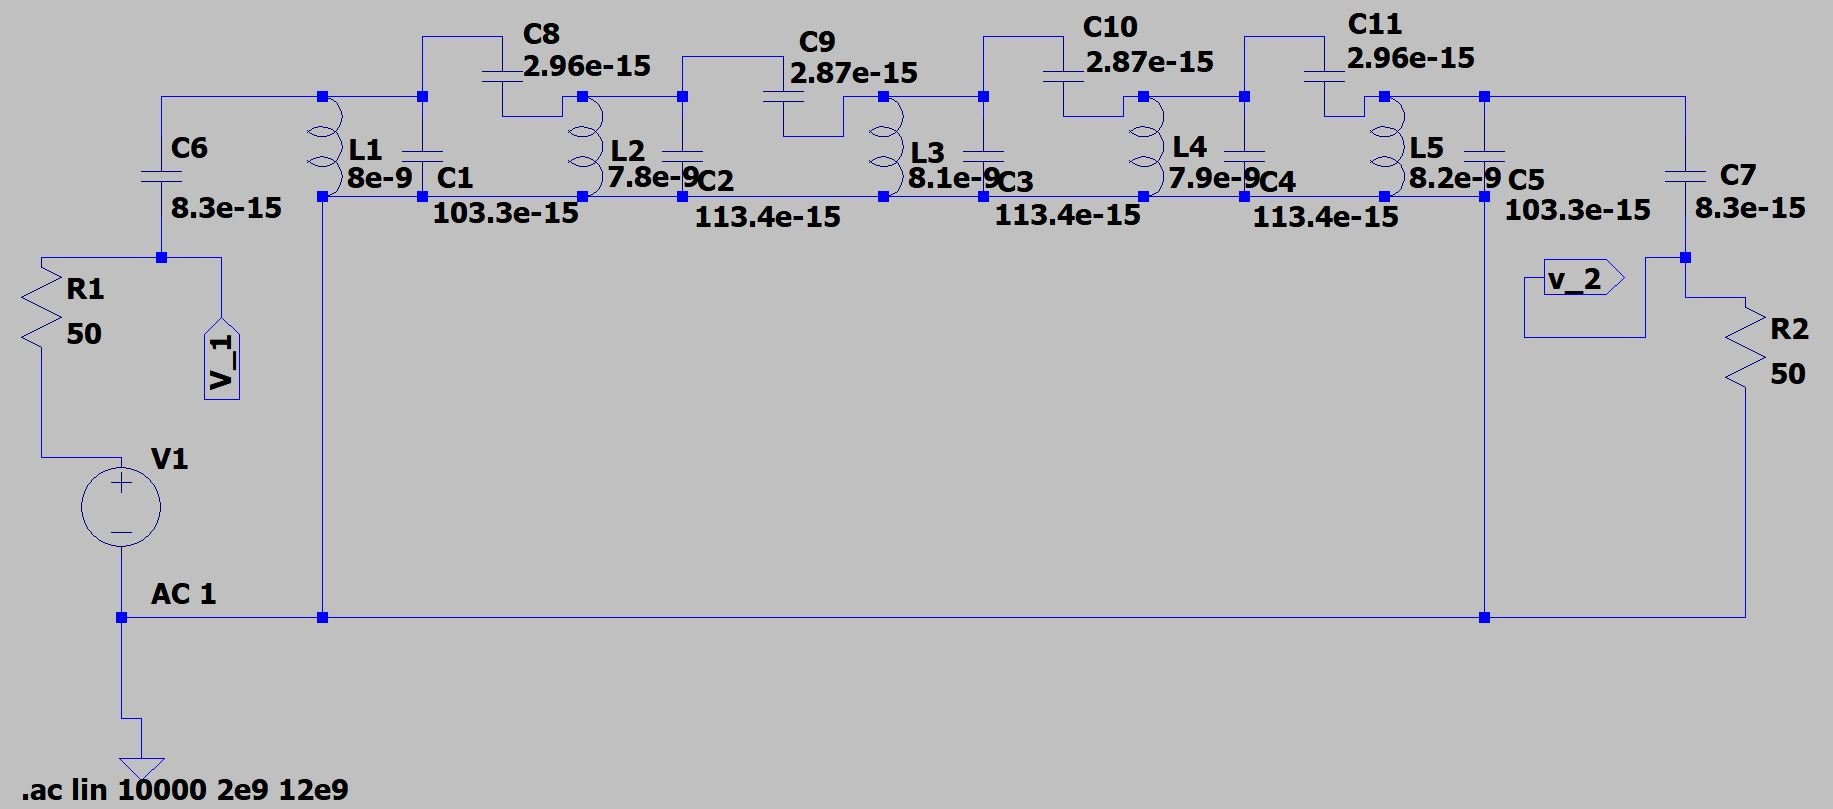
\includegraphics[width=\textwidth]{LTSpice_scheme_2}
	
	\begingroup
	\captionsetup[subfigure]{width=0.8\textwidth}
	\captionof{subfigure}{Electrical circut scheme in LTspice with different inductancies}
	\endgroup
	\end{minipage}
	\begin{minipage}{0.49\textwidth}
		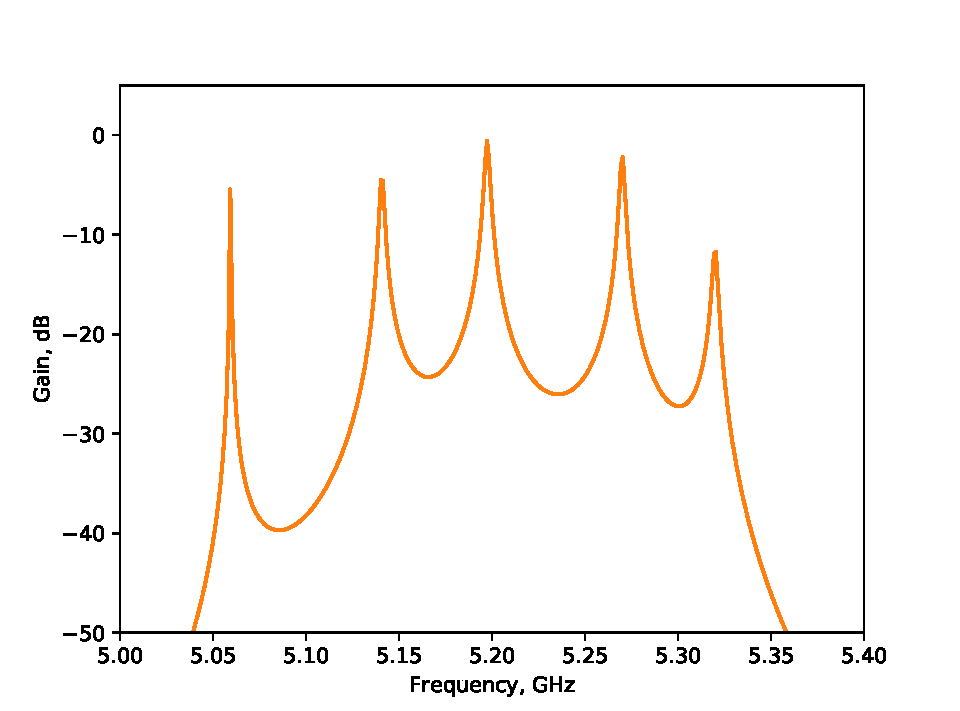
\includegraphics[width=\textwidth]{LTSpice_python_b_2}
		
		\begingroup
		\captionsetup[subfigure]{width=0.8\textwidth}
		\captionof{subfigure}{Classical mode frequencies in GHz: \{5.06, 5.142, 5.198, 5.271, 5.321\}}
		\endgroup
	\end{minipage}
	\centering
	\begin{minipage}{\textwidth}
		
		Using secular equation we calculated classical fluctuations:
		
	\end{minipage}

	\begin{minipage}{0.49\textwidth}
		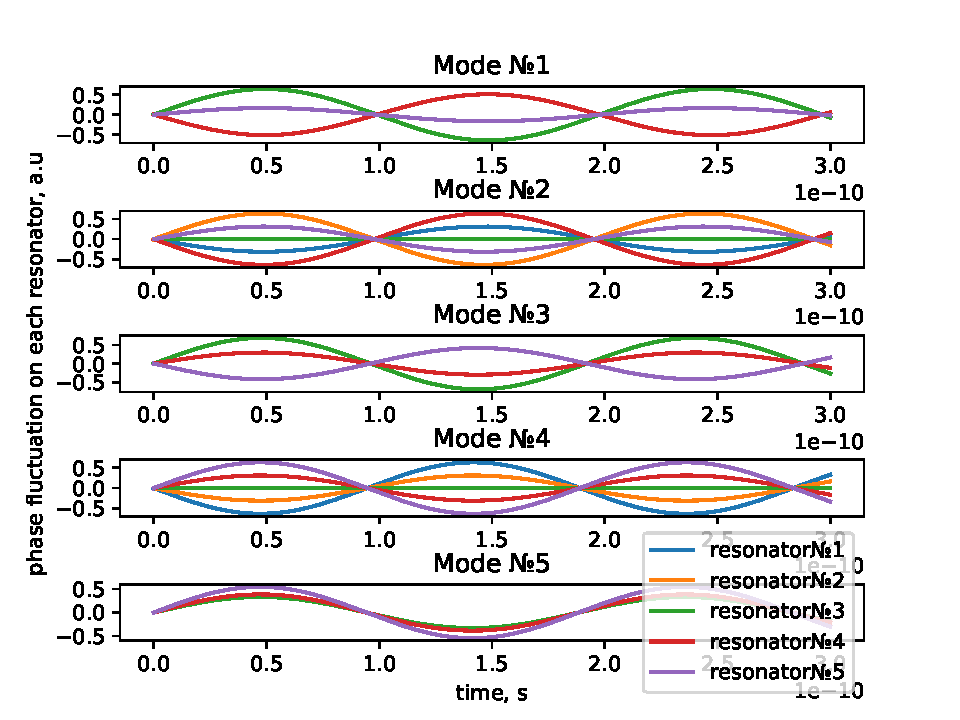
\includegraphics[width=\textwidth]{classical_modes}
		
		\begingroup
		\captionsetup[subfigure]{width=0.8\textwidth}
		\captionof{subfigure}{Classical modes.}
		\endgroup
	\end{minipage}
	\begin{minipage}{0.49\textwidth}
		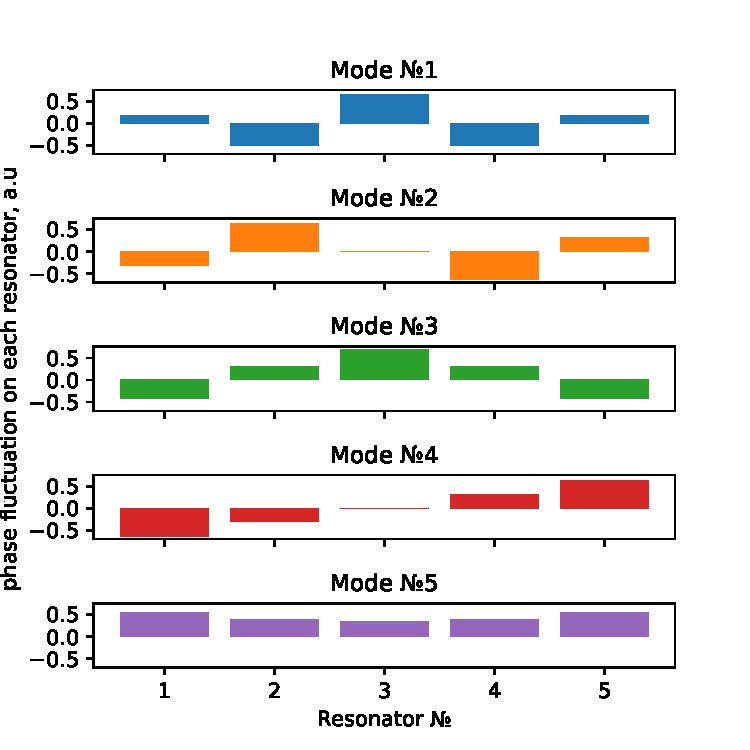
\includegraphics[width=\textwidth]{classical_modes_bar_chart}
		
		\begingroup
		\captionsetup[subfigure]{width=0.8\textwidth}
		\captionof{subfigure}{Fluctuation distribution at different modes at 0.05ns. Here we can see amplitudes and relative phases of fluctuations.}
		\endgroup
	\end{minipage}
	
\end{tcolorbox}


%%%%%%%Измерения
\tcbset{colframe=titlecol}
\begin{tcolorbox}[left=1cm, right=1cm, top=0.5cm, bottom=0.5cm, 
	title={\Large Dynamics simulation. Quantum approach}, bottomtitle=.3cm,toptitle=.5cm
	]
	\begin{minipage}{\textwidth}
		
		Calculated quantum chain frequencies in GHz:\{4.893,4.957,5.041,5.116,5.129\}.
		Using Lindblad Master Equation Solver in QuTiP we can simulate chain dynamics by applying drive with one of modes frequency (see Fig.5).
		$H_{drive} = f(t)\hat{n}_1\otimes \hat{1}\otimes \hat{1}\otimes \hat{1}\otimes \hat{1} $, where
		$f(t)=\hbar f\theta(t-begin)\theta(begin+t_{exc}-t)\sin \left(\omega_{drive} t + \varphi\right)$
		
	\end{minipage}

	\vspace{1cm}
	\begin{minipage}{0.49\textwidth}
		\centering
		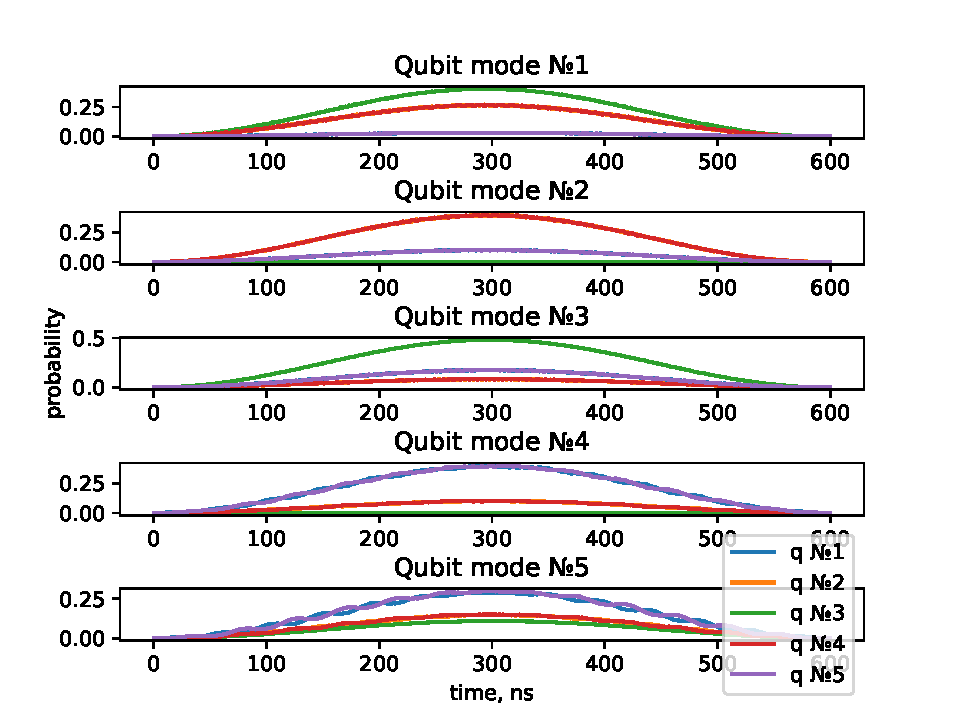
\includegraphics[width=\textwidth]{quantum_dynamics}
		\begingroup
		\captionsetup[figure]{width=\textwidth}
		
		\captionof{figure}{Chain dynamics. Probability means squared projection on $|00..i..00>$ state for each qubit. 2nd and 4th lines merge into one as well as 1st and 5th.}
		\endgroup
	\end{minipage}
	\begin{minipage}{0.49\textwidth}
	\centering
	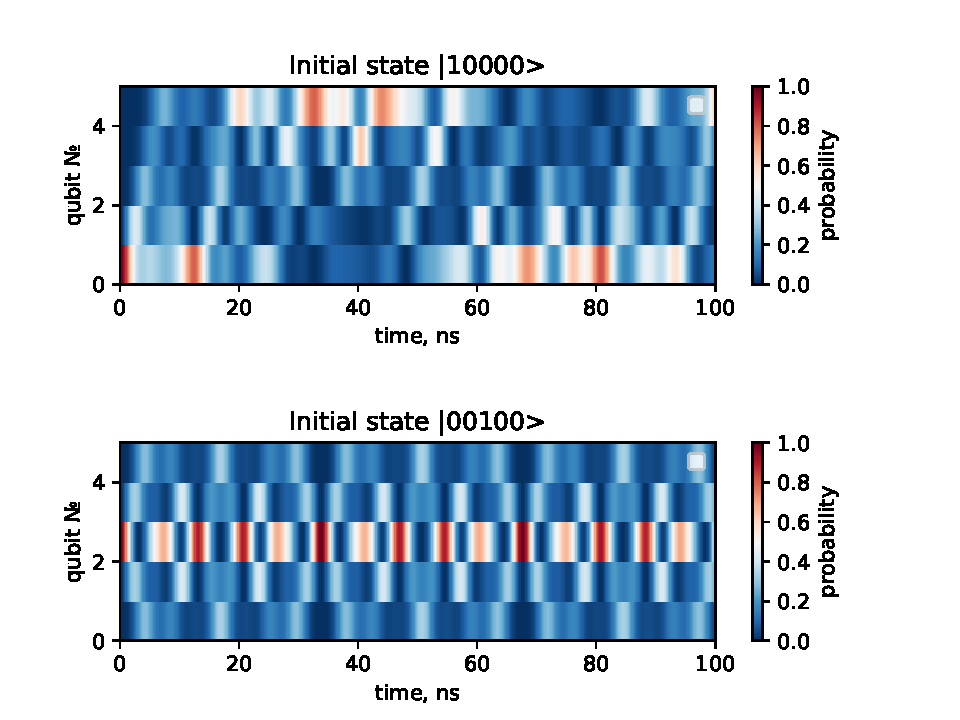
\includegraphics[width=\textwidth]{quantum_dynamics_3d}
	\begingroup
	\captionsetup[figure]{width=\textwidth}
	
	\captionof{figure}{The time evolution of excitation distribution after the initially localized state by placing one microwave photon into 1st or 3rd qubit. Probability means squared projection on $|00..i..00>$ state for each qubit.}
	\endgroup
	\end{minipage}

	

\end{tcolorbox}

%%%%%%%% Conclusion

\tcbset{colframe=titlecol}
\begin{tcolorbox}[left=1cm, right=1cm, top=0.5cm, bottom=0.5cm, 
                  title={\Large Conclusion}, bottomtitle=.5cm,toptitle=.5cm
                  ]

In this paper, we designed and investigated a chain of five transmons. Through modeling, it is shown that this design is suitable for simulating the Ising model. We are looking forward to the opportunity of making an experiment.

\end{tcolorbox}

\tcbset{colframe=titlecol}
\begin{tcolorbox}[left=1cm, right=1cm, top=0.5cm, bottom=0.5cm, 
                  title={\Large Referencies}, bottomtitle=.5cm,toptitle=.5cm
                  ]
\bibliography{poster2019.bib}

\end{tcolorbox}

\end{multicols}


\end{document}